\section{Selected Amanzi libraries}

This section describes Amanzi libraries, their limitations and possible 
ways to extend.

\subsection{WhetStone}
This is a low-level library that implements primarily local matrices for 
various discretizations schemes. 
Conceptual dosing of this part of the library is presented in Fig.~\ref{fig:whetstone}.
Classes derived from class {\tt MFD3D} cover a huge spectrum of elliptic
operators.

Additional functionality included in this library supports
\begin{enumerate}
\item the ring algebra of scalar, vector and matrix polynomials;
\item quadrature rules on simplices;
\item numerical integration algorithms based on the Euler homogeneous theorem;
\item coordinate transformations including parameterization of mesh faces and edges.
\end{enumerate}

A few  comments on the design principles. 
Polynomial coefficients are represented by a linear array. 
An polynomial iterator class allow us to access information about monomial terms of 
a given polynomial in a for-type loop:
\begin{lstlisting}
Polynomial poly(3, 2);
for (auto it = poly.begin(); it < poly.end(); ++it) {
  int i = it.PolynomialPosition();
  int k = it.MonomialSetOrder();
  const int* idx = it.multi_index();
  double ci = poly(i);
}
\end{lstlisting}
Each step of this loop extracts information about monomial $c_i \,x^{idx_0} y^{idx_1} z^{idx_2}$
of order $k= idx_0 + idx_1 + idx_2$ in a quadratic polynomial.

Quadrature rules on simplexes have positive weights for stability of numerical schemes. 
Integration formulas based on Euler's homogeneous theorem can be used for integrating
polynomials over polytopal cells.
To integrate polynomial and non-polynomial functions using a single interface a simple
base class {\tt WhetStoneFunction} is used.

Coordinate transformation allows us to treat a 3D mesh face as a 2D polygon.
This is used in (a) hierarchical construction of high-order virtual element and mimetic 
schemes, and (b) projection of polynomials on a low-dimension manifold and an reserve (non-unique)
lifting operation.

Finally library {\it WhetStone} contains a factory of discretization schemes that could
be extended by including users schemes via simple interface.
Example of such an extension is available in Operator's tests.


\begin{figure}[h!]
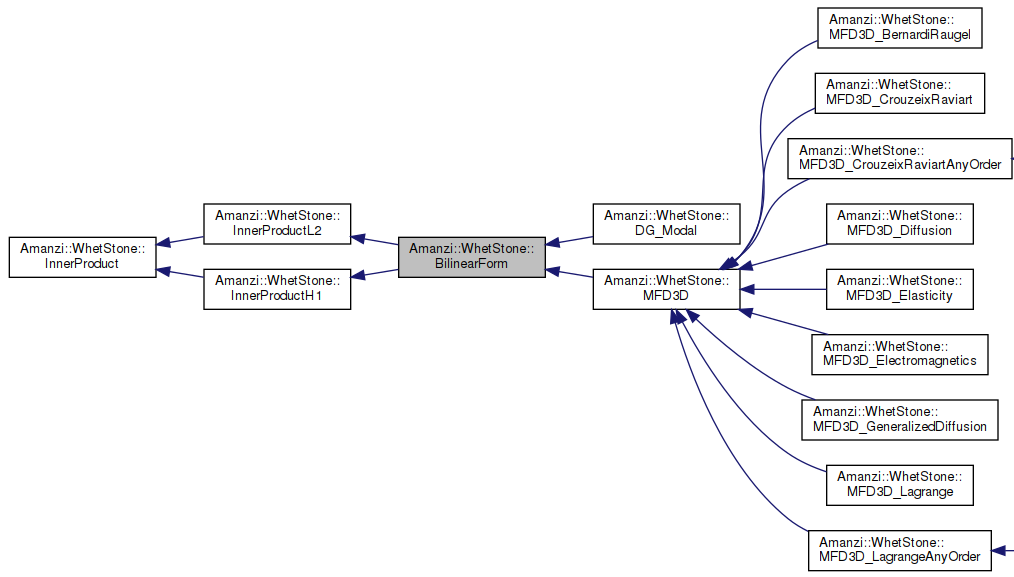
\includegraphics[width=1.0\textwidth]{figs/whetstone.png}
\caption{Partial dependency tree for library WhetStone.\label{fig:whetstone}}
\end{figure}

\clearpage
\subsection{Operators}

\begin{figure}[h!]
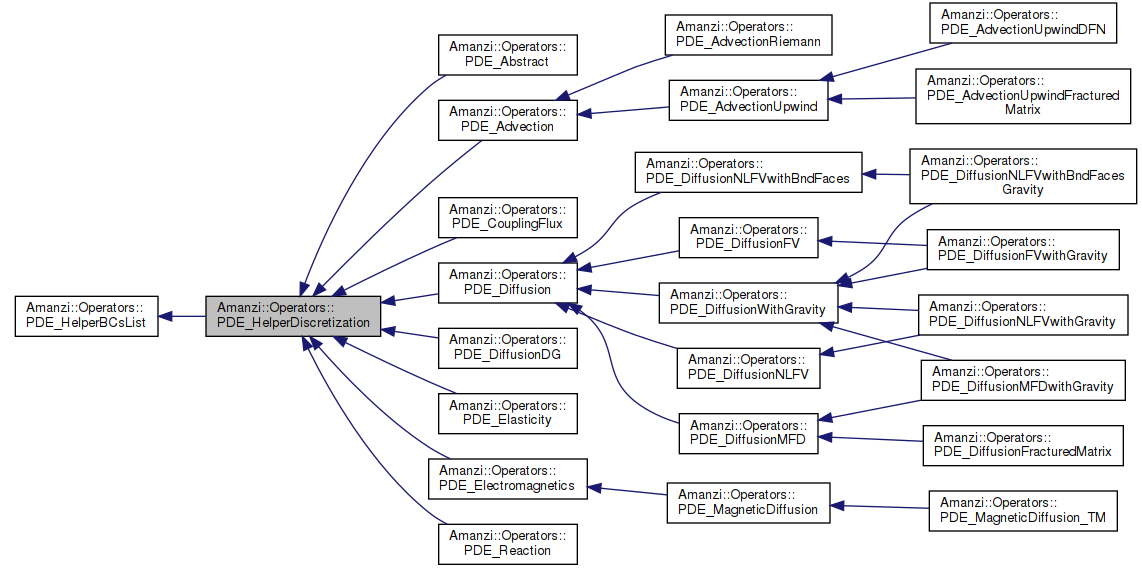
\includegraphics[width=1.0\textwidth]{figs/operators.png}
\caption{Partial dependency tree for library Operators.\label{fig:operators}}
\end{figure}


\subsection{PKs}

Bla-bla-bla

